% !TEX root = PREN2_Dokumentation.tex
\section{Methoden}
\subsection{\gls{SoDa}}
Das Projektmanagement wird mit dem hybriden Projektvorgehen \gls{SoDa} der Hochschule Luzern durchgeführt. 
\gls{SoDa} wurde dabei bereits schon in vorhergehenden Softwareentwicklungsmodulen eingesetzt und hat sich hier bewährt. Die Userstories werden dabei auch im \gls{GitLab} erfasst.  
\begin{figure}[H]
	\centering
	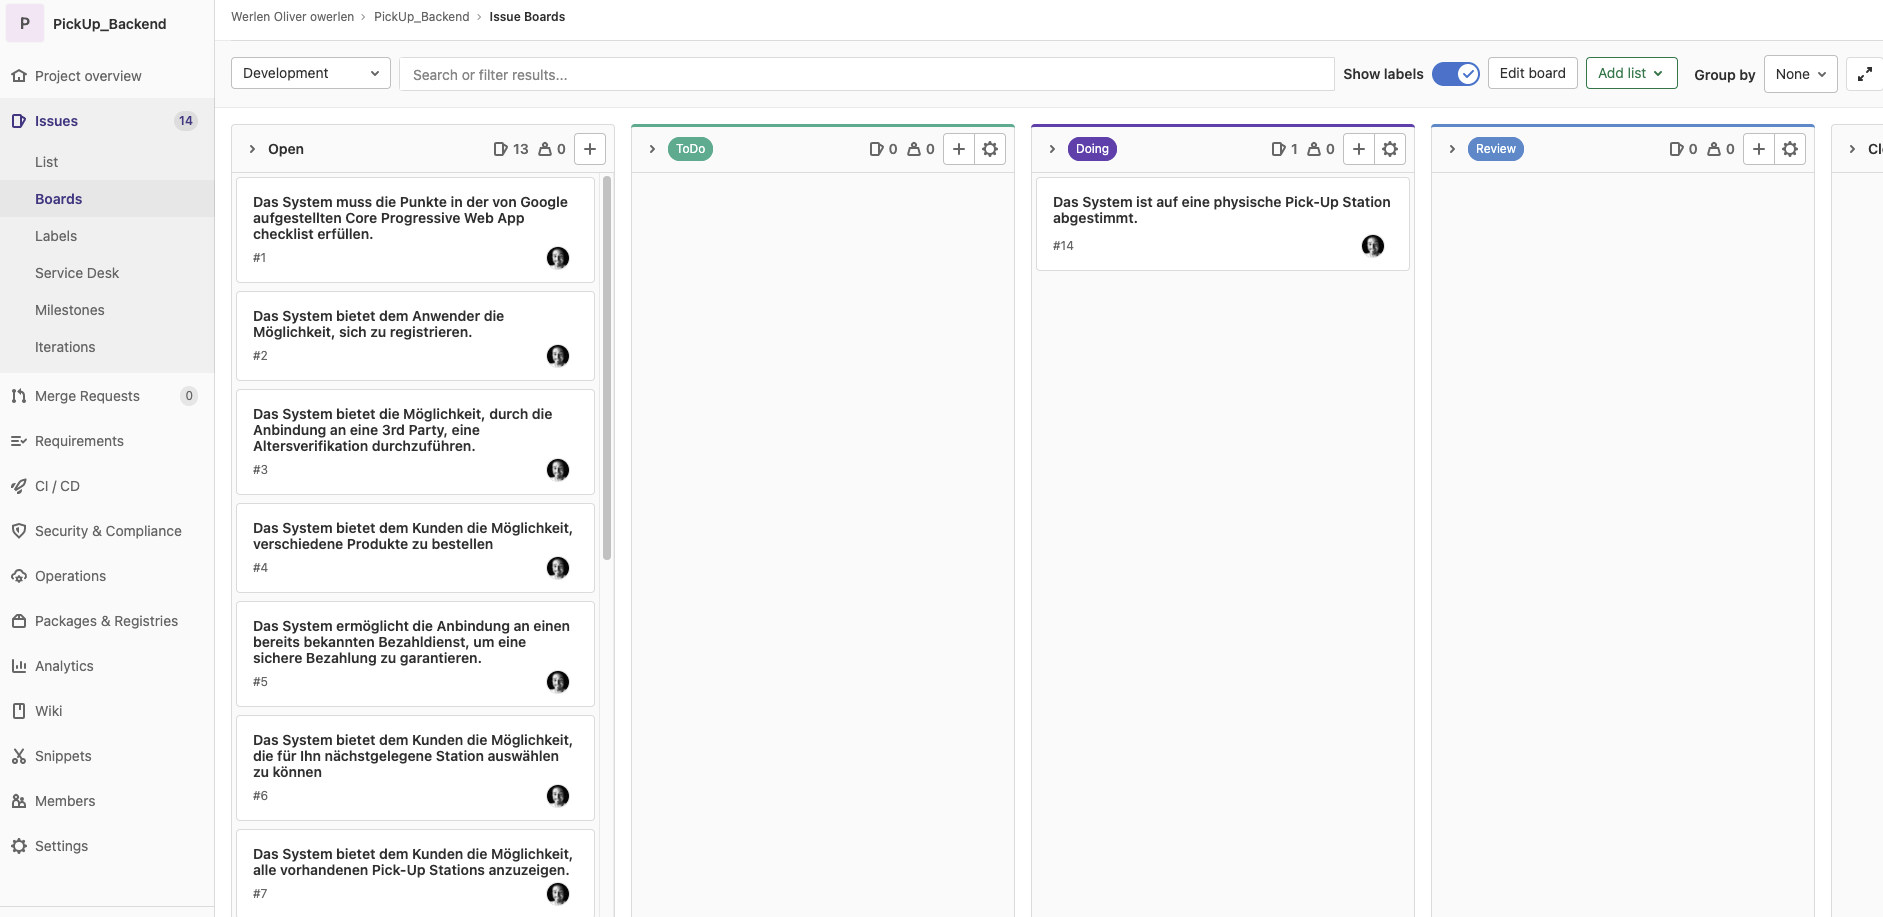
\includegraphics[scale=0.5]{images/boardGitlab.png}
	\caption[GitLab Board]{GitLab Board,\\ Quelle: Autor}
	\label{img: GitlLabBoard}
\end{figure}
Beim Sprint Review werden die Stories in reviewing mit den definierten Akzeptanzkriterien mit den Resultaten verglichen. Basierend darauf wird entschieden, ob an der \gls{User Story} noch weiter gearbeitet werden, das heisst zurück zu doing oder die Story in done verschoben werden kann. Bei Beginn des nächsten Sprints wird das Vorgehen wiederholt. \\
Die einzelnen Items sind dabei priorisiert. Elemente mit einer hohen Einstufung werden dabei bei der Bearbeitung vorgezogen. 

\subsection{Domain Driven Design}
Domain Driven Design ist eine Herangehensweise an die Erstellung von komplexer Software. Sie befasst sich in den meisten Fällen mit Businessproblemen. Dieses Problem wird als Domäne bezeichnet. Die Software ist von Beginn an und durchgängig mit dieser Domäne verknüpft. \\
Als Domäne wurde in diesem Projekt der Verkauf und die Abholung von Tabakprodukten identifiziert [\cite{domainDrivenDesign}]. 

\subsubsection{Aufbau von Domain-Knowledge}
Um ein Domain-Wissen aufzubauen, wurde während dem gesamten Projekt enger Kontakt mit den Kontaktpersonen von \ac{JTI} gepflegt. Besonders in der Initialisierungsphase wurde das Businessproblem besprochen und durch die Recherche von artverwandten Technologien erweitert. 
Als Resultat wurde die folgende Domäne erstellt: 
\begin{figure}[H]
	\centering
	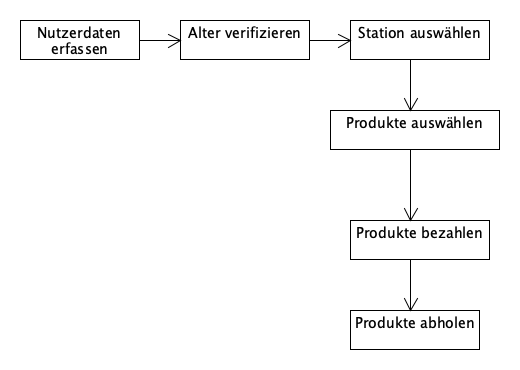
\includegraphics[scale=0.5]{images/Domain.png}
	\caption[Domänenmodell]{Domänenmodell, Quelle: Autor}
	\label{img: domain}
\end{figure}

\subsubsection{Model Driven Design}
Das erstellte Modell ist sehr stark mit der Domäne verknüpft. Basierend darauf wurde die Software designed und implementiert. Domain Driven Design setzt auf verschiedenste Pattern.  
\paragraph{Entities}\label{entity}
Eine Entity hat immer eine Identität. Kann im System eindeutig identifiziert werden. Nicht alle Objekte in einem System sind Entities. Entities sind ressourcenintensiv, da immer sichergestellt werden muss, dass die Entity einzigartig ist.
\paragraph{Value Objects}
Es ist nicht in jedem Anwendungsfall nötig, das gesamte Objekt zu erhalten. Ein Value Objekt ist ein Objekt, welches nur einen Teilbereich aus einer Domäne beschreibt. Ohne eine Entity sind Value Objects sehr leichtgewichtig. \\
Es wird sehr stark empfohlen, Value Objects Immutable zu machen. \\
Value Objects können zudem Referenzen zu anderen Objekten enthalten. \ac{DTO}'s entsprechen Value Objects. 

\paragraph{Services}\label{services}
Der Service bearbeitet Value Objects oder Entities. Dabei hat er drei Eigenschaften: 
\begin{enumerate}
	\item Der Service gehört zu einem Domänenkonzept, welches nicht direkt zum Domänenobjekt gehört.
	\item Die Operation verweist auf andere Objekte in der Domäne.
	\item Die Operation ist statuslos. 
\end{enumerate}

\paragraph{Repositories}
Das Repository entkapselt die Persistierung von Objekten und bildet somit die Schnittstelle zwischen Applikation und Datenbank. 

\subsection{CI/CD}
Die gesamte \ac{CI/CD} Pipeline wurde für dieses Projekt neu erstellt. Dabei besteht der Prozess aus drei Stages: 
\begin{enumerate}
	\item build
	\item package
	\item deploy
\end{enumerate}

\subsubsection{build}
Abhängig vom Projekt wird das Projekt gebuilded. Bei der Java Applikation handelt es sich hier um ein maven-package, beim Angular Frontend um ein \glqq ng build -prod\grqq{}. Die resultierenden Artifakte werden für zwei Stunden im GitLab gespeichert. 
\subsubsection{package}
In der Package Stage wird das Docker Image aus den vorherigen Artifakten erstellt. Dabei wird das Dockerfile des jeweiligen Produkts genutzt. Der Build wird von einem Shared Runner durchgeführt. Hier werden 4 vom Enterpriselab zur Verfügung gestellt. Anschliessend wird dieses in die Container Registry des GitLab Projekts gepushed. 
\subsubsection{deploy}
Für das Deployment wurde auf den virtuellen Maschinen ein GitLab Runner installiert. Durch den deployment-Tag wird dieser adressiert. Auf diese Maschine wird ein Login ausgeführt und anschliessend das aktuellste Image heruntergeladen. Es wird der bestehende Container gelöscht und aus dem neuen Image ein neuer Container gestartet. 

\subsubsection{Sequenzdiagramm}
\begin{figure}[H]
	\centering
	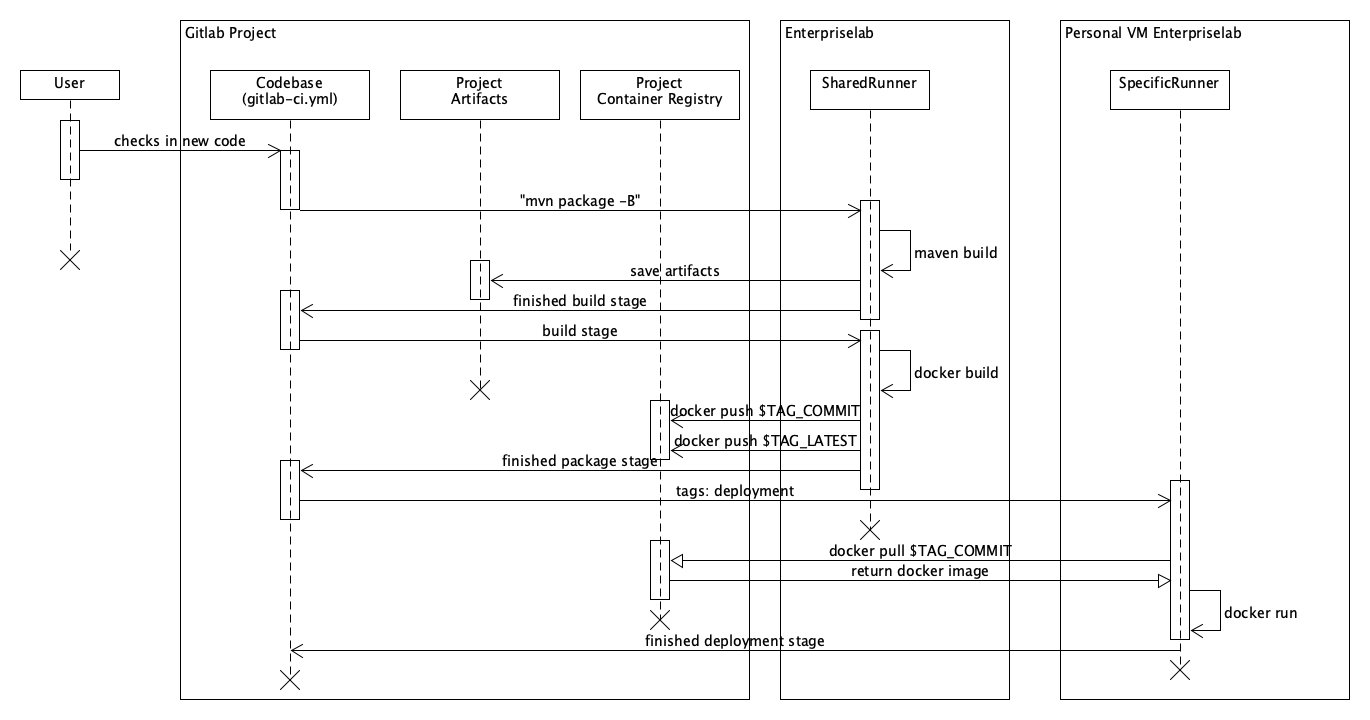
\includegraphics[width=1\textwidth]{images/sequenceCicd.png}
	\caption[Ablauf der CI/CD Pipeline]{Ablauf der CI/CD Pipeline, Quelle: Autor}
	\label{img: cicdPipeline}
\end{figure}


\subsubsection{Testing}
Das Projektziel ist ein Prototyp. Aus diesem Grund wurde der Fokus auf die Funktion gesetzt. Daher wurden die Unit- und Integrationstests nur konzeptuell umgesetzt. Bei Bedarf können diese erweitert werden. 

\newpage